\documentclass[a4paper,10pt,american]{article}
\usepackage[top=1in, bottom=1in, left=0.75in, right=0.75in]{geometry}
\usepackage{amsmath,amssymb,amsfonts,mathrsfs,accents} %important math packages
\usepackage{graphicx}
\usepackage{subcaption}
% \usepackage{float}
\usepackage{bbm}
\usepackage{dsfont}
\usepackage{tikz}
\usepackage{enumerate} % package for making different lists
\usepackage[T1]{fontenc} % Encoding of fonts
\usepackage{lmodern} % Latin modern font - needed for fontenc
\usepackage[utf8]{inputenc} % Encoding of input text
\usepackage[kerning]{microtype} % Better looking text
\usepackage[babel]{csquotes} % Better looking quotes
\usepackage{booktabs} % Better looking tables
\usepackage{babel} % Language control, for hyphenation etc
\usepackage{amsthm} % Package for theorem and definition environments
\usepackage{hyperref} % URLs 
\usepackage{comment}
\usepackage{xcolor}
\usepackage{amsmath}
\usepackage[table]{xcolor}
\usetikzlibrary{trees}
\usepackage{istgame}
\usepackage{mathpazo} % Other fonts: lmodern & charter & mathptmx
% \usepackage{minted}
% \usemintedstyle{colorful}  % Choose a highlighting style
\usepackage{listings}
% Package for drawing in Latex. Depending on your installation you might need compat=1.12 or 1.11 uncommented.  
\usepackage{tikz}
\usetikzlibrary{calc}
\usepackage{pgfplots}
\usepackage{fancyhdr}
\usepackage{footmisc}
%\pgfplotsset{compat=1.12}
\pgfplotsset{compat=1.11}

% For better figure placement in documents. Use [H] instead of the usual [htbp]. Inserted at the same place as in the code, as you normally want it to. 
\usepackage{float}

% Row break instead of indent for new paragraph. 
\usepgfplotslibrary{fillbetween}
\setlength{\parskip}{10pt plus 1pt minus 1pt}
\setlength{\parindent}{0in}

% Define Stata language style
\lstdefinelanguage{Stata}{
    morekeywords={regress, gen, summarize, predict, display, if, forval, local, matrix},
    sensitive=true,
    morecomment=[l]{*},
    morestring=[b]",
}
% Set listings style
\lstset{
    language=Stata,
    basicstyle=\ttfamily\small,    % Code font
    keywordstyle=\color{blue},    % Keywords in blue
    commentstyle=\color{gray},    % Comments in gray
    stringstyle=\color{red},      % Strings in red
    breaklines=true,              % Allow line breaking
    numbers=left,                 % Line numbers on the left
    numberstyle=\tiny\color{gray},
    frame=single,                 % Frame around the code
    captionpos=b,                 % Caption position
}
% Examples of personal commands to simplify writing stuff you use often. 
\newcommand{\reals}{\mathbb{R}} 
\newcommand{\rtwo}{\mathbb{R}^2}
\newcommand{\ints}{\mathbb{Z}}
\newcommand{\nats}{\mathbb{N}}
\newcommand{\matset}{\mathcal{M}}
\newcommand{\zerovec}{\{\mathbf{0}\}}
% \renewcommand{\footnoterule}{%
%     \kern 210pt
%     \hrule width \textwidth height 0.4pt
%     \kern 2.6pt
% }
\definecolor{navy}{RGB}{0, 0, 128}
\hypersetup{
    colorlinks=true,
    linkcolor=navy,
    filecolor=navy,
    urlcolor=navy,
    citecolor=navy,
}
\title{ASSET PRICING THEORY --- Problem Set 3}
\author{Ali Bahramisani\thanks{Stockholm School
of Economics, Department of Finance, Email: 
\href{mailto:ali.bahramisani@hhs.se}{ali.bahramisani@hhs.se}, 
Website: \href{https://alibahramisani.github.io}{alibahramisani.github.io}},
Alfred Bornefalk\thanks{Stockholm School
of Economics, Department of Finance, Email: 
\href{mailto:alfred.bornefalk@hhs.se}{alfred.bornefalk@hhs.se}}}

\date{Spring 2025}

\pagestyle{fancy}
\fancyhf{}
\fancyhead[L]{A. Bahramisani, A. Bornefalk}
\fancyhead[C]{Asset Pricing Theory- Spring 2025}
\fancyhead[R]{Problem Set 3}
\fancyfoot[C]{\thepage}
% \setlength{\abovecaptionskip}{0pt}
% \setlength{\belowcaptionskip}{0pt}

\usepackage{natbib}
\bibliographystyle{abbrvnat}
\setcitestyle{authoryear,open={(},close={)}}

\begin{document}
\maketitle
\vspace{1cm}
    \begin{center}
        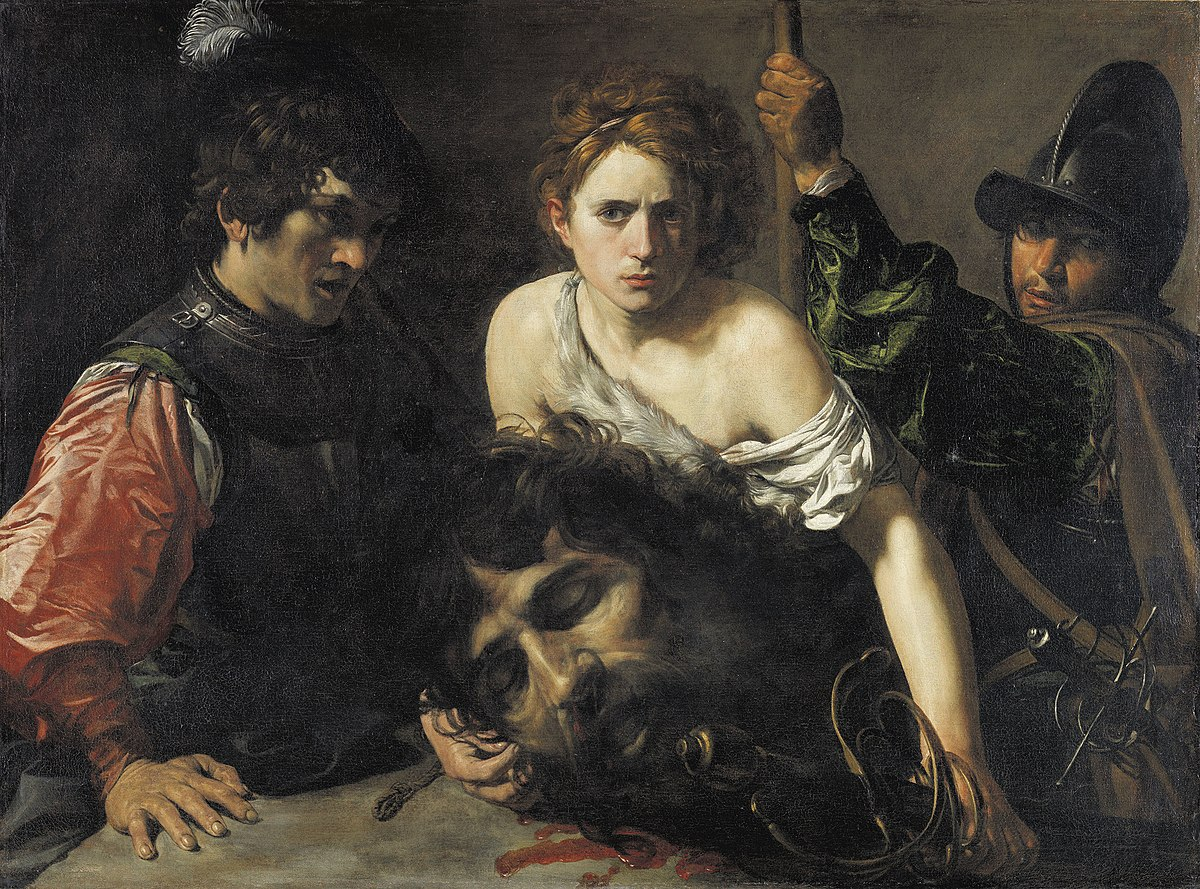
\includegraphics[width=0.9\textwidth]{DG.jpg} \\[1ex]
        {\footnotesize \textit{David With the Head of Goliath and two Soldiers} \citep{valentin_boulogne_david}. 
        David outperformed his large enemy, but at a great risk.}
    \end{center}
    \vfill
% \thispagestyle{empty}



\newpage
\pagenumbering{arabic}

\section*{Exercise (\textit{i})}
\subsection*{Rationale for the Two Adjustments}
\subsubsection*{Adjustment for Returns (Delisting Returns)}
When a stock is delisted, shareholders may still receive some return 
(e.g., from a merger or acquisition). This return is not captured in the
\texttt{dlret} variable in CRSP. By adjusting the last recorded return 
(\texttt{ret}) to include the delisting return (\texttt{dlret}), 
we account for the final payoff to shareholders. The formula
$(1+R_{adj}) = (1+R_{normal})\times (1+R_{delist})$ ensures that the
adjusted return reflects the total return, including the delisting event.
Overall, this adjustment ensures that the dataset accurately reflects the 
performance of all stocks, including those that are delisted, removing the 
potential downward bias in portfolio returns.


\subsubsection*{Adjustment for Survivor Bias (Two-Year Rule)}
By excluding firms until they have appeared on COMPUSTAT for two years,
we ensure that our dataset includes only firms that have survived long 
enough to be reliably tracked. This reduces the bias introduced by 
excluding firms that fail early and provides a more accurate representation
of the population of firms.This adjustment ensures that the dataset is not 
biased towards firms that have already demonstrated some level of 
survivability, providing a more accurate and representative sample 
for analysis.

\subsection*{Share of Stocks in Each Portfolio over Time}

\autoref{fig:SPOSPT} shows the share of portfolios over time. The share of
the portfolios is relatively stable over time.

\begin{figure}[H]
\centering
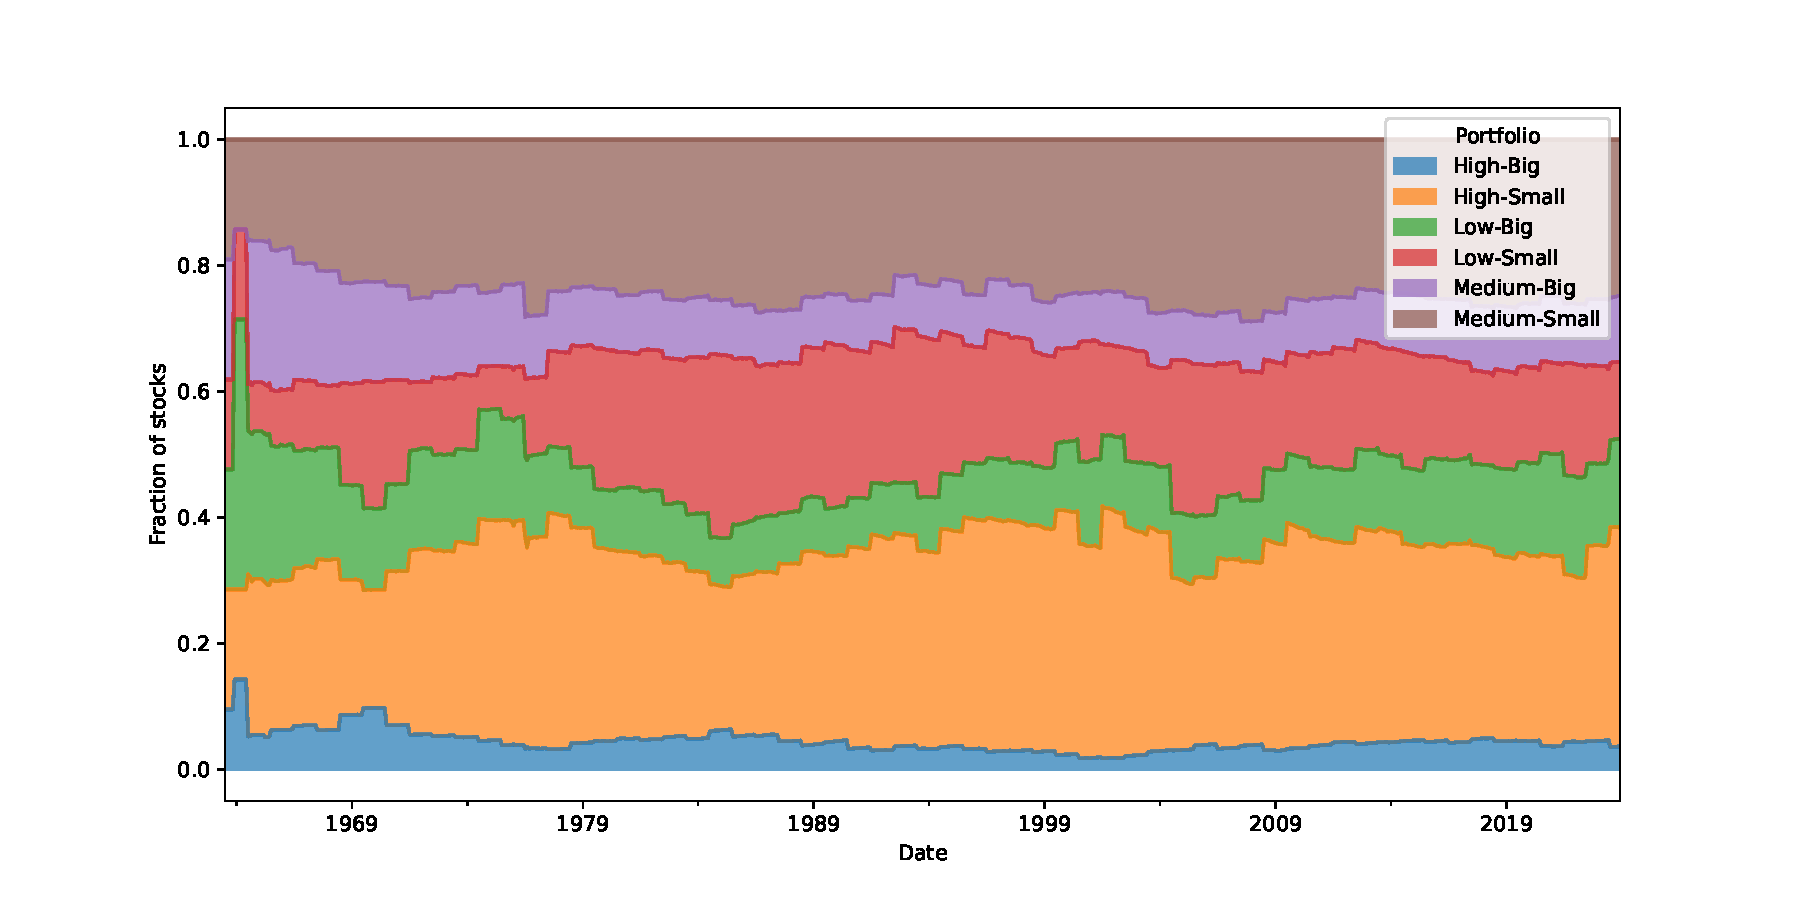
\includegraphics[width=1\linewidth]{../Plots/portfolio_shares_v2.pdf}
\caption{Share of the Six Portfolios Over Time.}
\label{fig:SPOSPT}
\end{figure}

\autoref{fig:VWSP} shows the value-weighted returns of the six portfolios.
They are generally fluctuating in the $\pm 20$ percent over time. The returns
of the \textit{Low Small} and \textit{High Small} portfolios are more
volatile than the other portfolios.

\begin{figure}[H]
\centering
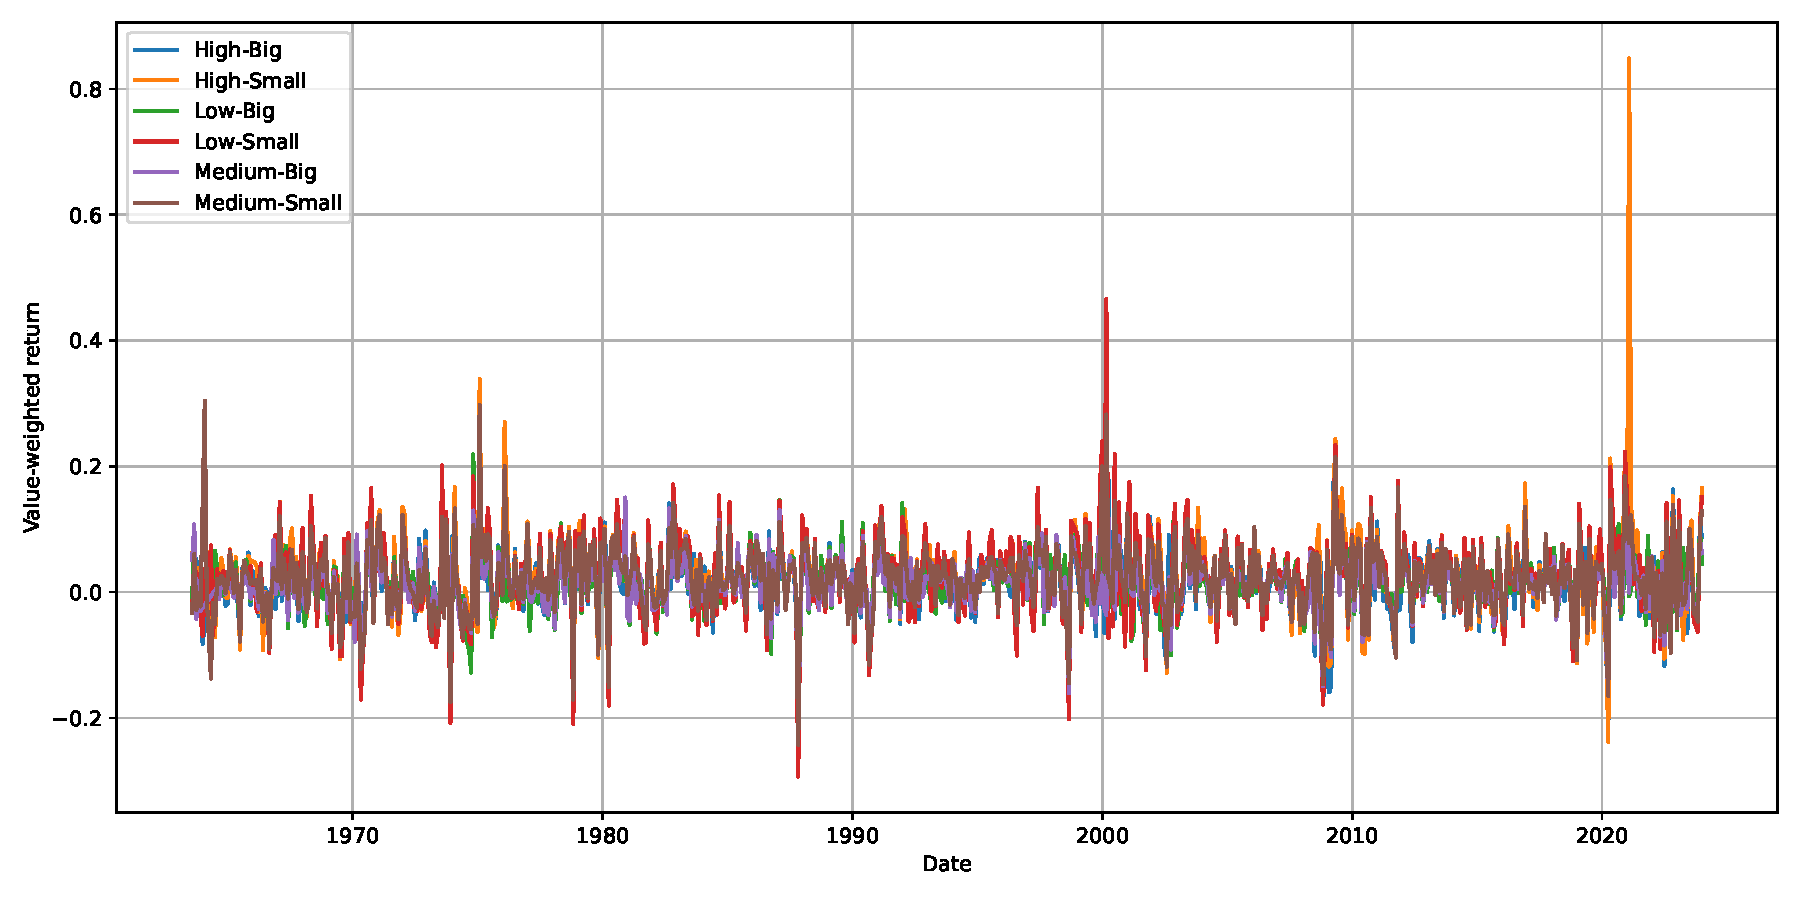
\includegraphics[width=1\linewidth]{../Plots/vw_returns_six_portfolios.pdf}
\caption{Value Weighted Returns of the Six Portfolios.}
\label{fig:VWSP}
\end{figure}

\subsection*{Rationale for the Construction of Book-to-Market Portfolios}

Look-ahead bias occurs when future information (not available at the time
 of portfolio formation) is inadvertently used in the analysis. 
 \cite{fama1992cross}'s methodology avoids this bias in the following ways:
\begin{enumerate}
    \item The book-to-market ratio is calculated using the lagged data 
    (e.g., December 1979 data is used to form portfolios in June 1980).
    This ensures that the information used to construct portfolios is
    available to investors at the time of portfolio formation.
    \item Portfolios are formed in June and held until the following June. 
    This ensures that the returns are calculated using only information
    available at the time of portfolio formation.
    \item The methodology does not rely on any future data (e.g., 
    future returns or financials) to construct portfolios, ensuring 
    that the results are free from look-ahead bias.
\end{enumerate}

\cite{bowles2024anomaly} show that the conventional method of portfolio rebalancing
used in financial research leads to anomaly portfolios that rely on information that
can be severely outdated. Hence, it can be argued that the June rebalancing approach by 
\cite{fama1992cross}, while avoiding look-ahead bias, introduces staleness bias.

\subsection*{Discrepancy with Fama French (Importing other data)}

We see from \autoref{fig:RDBFVP} that the time series of our return
differences and French's, while being arguably similar, still are far 
away from being perfect matches. In particular, from \autoref{fig:CRFVP}, 
we see that our portfolios have consistently higher cumulative returns 
than French's. One major reason as to why our results differ is that 
\cite{fama1992cross} exclude financial firms from their portfolio constructions, 
which we have not. Indeed, if financial firms then overperformed during our 
sample period, this would explain part of the difference. For instance, 
we see that in the times of crises, i.e., the IT bubble, the Great 
recession, and during the start of the Covid-19 pandemic, some of our 
portfolios have far greater returns than their French counterparts,
which could be an artifact of the different portfolio 
compositions. Ceteris paribus, this could then explain the differences 
in cumulative returns.

\begin{figure}[H]
\centering
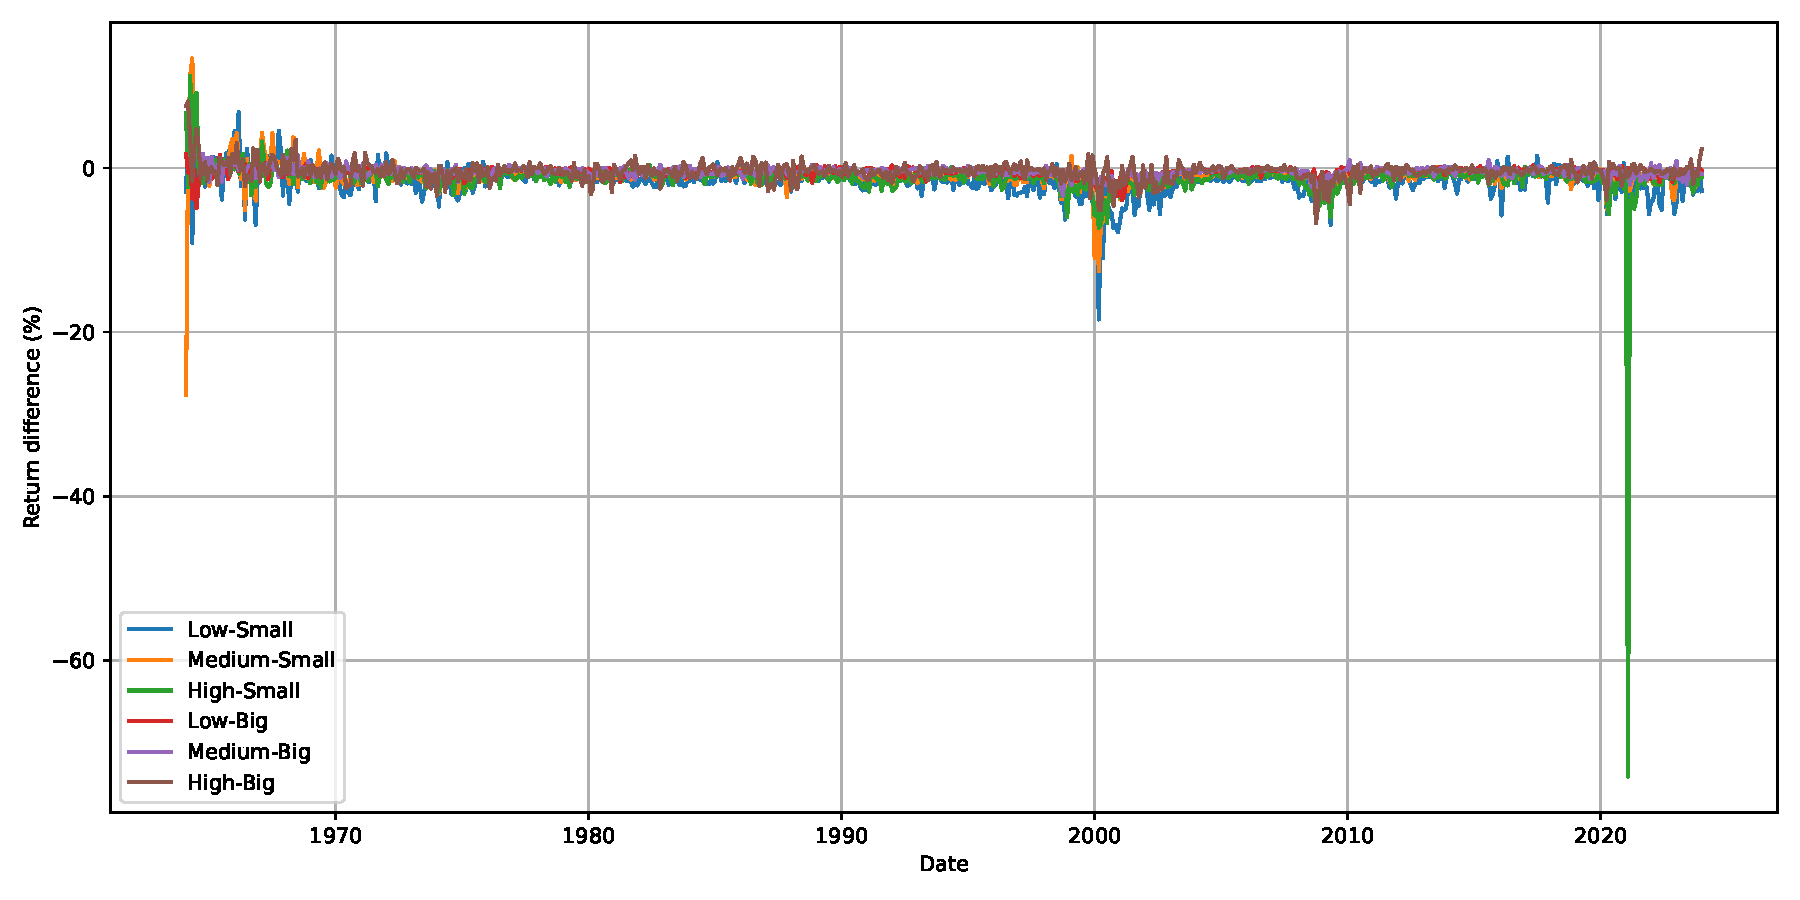
\includegraphics[width=1\linewidth]{../Plots/return_diff.pdf}
\caption{Return Differences Between French and Value-Weighted Portfolios.}
\label{fig:RDBFVP}
\end{figure}


\begin{figure}[H]
\centering
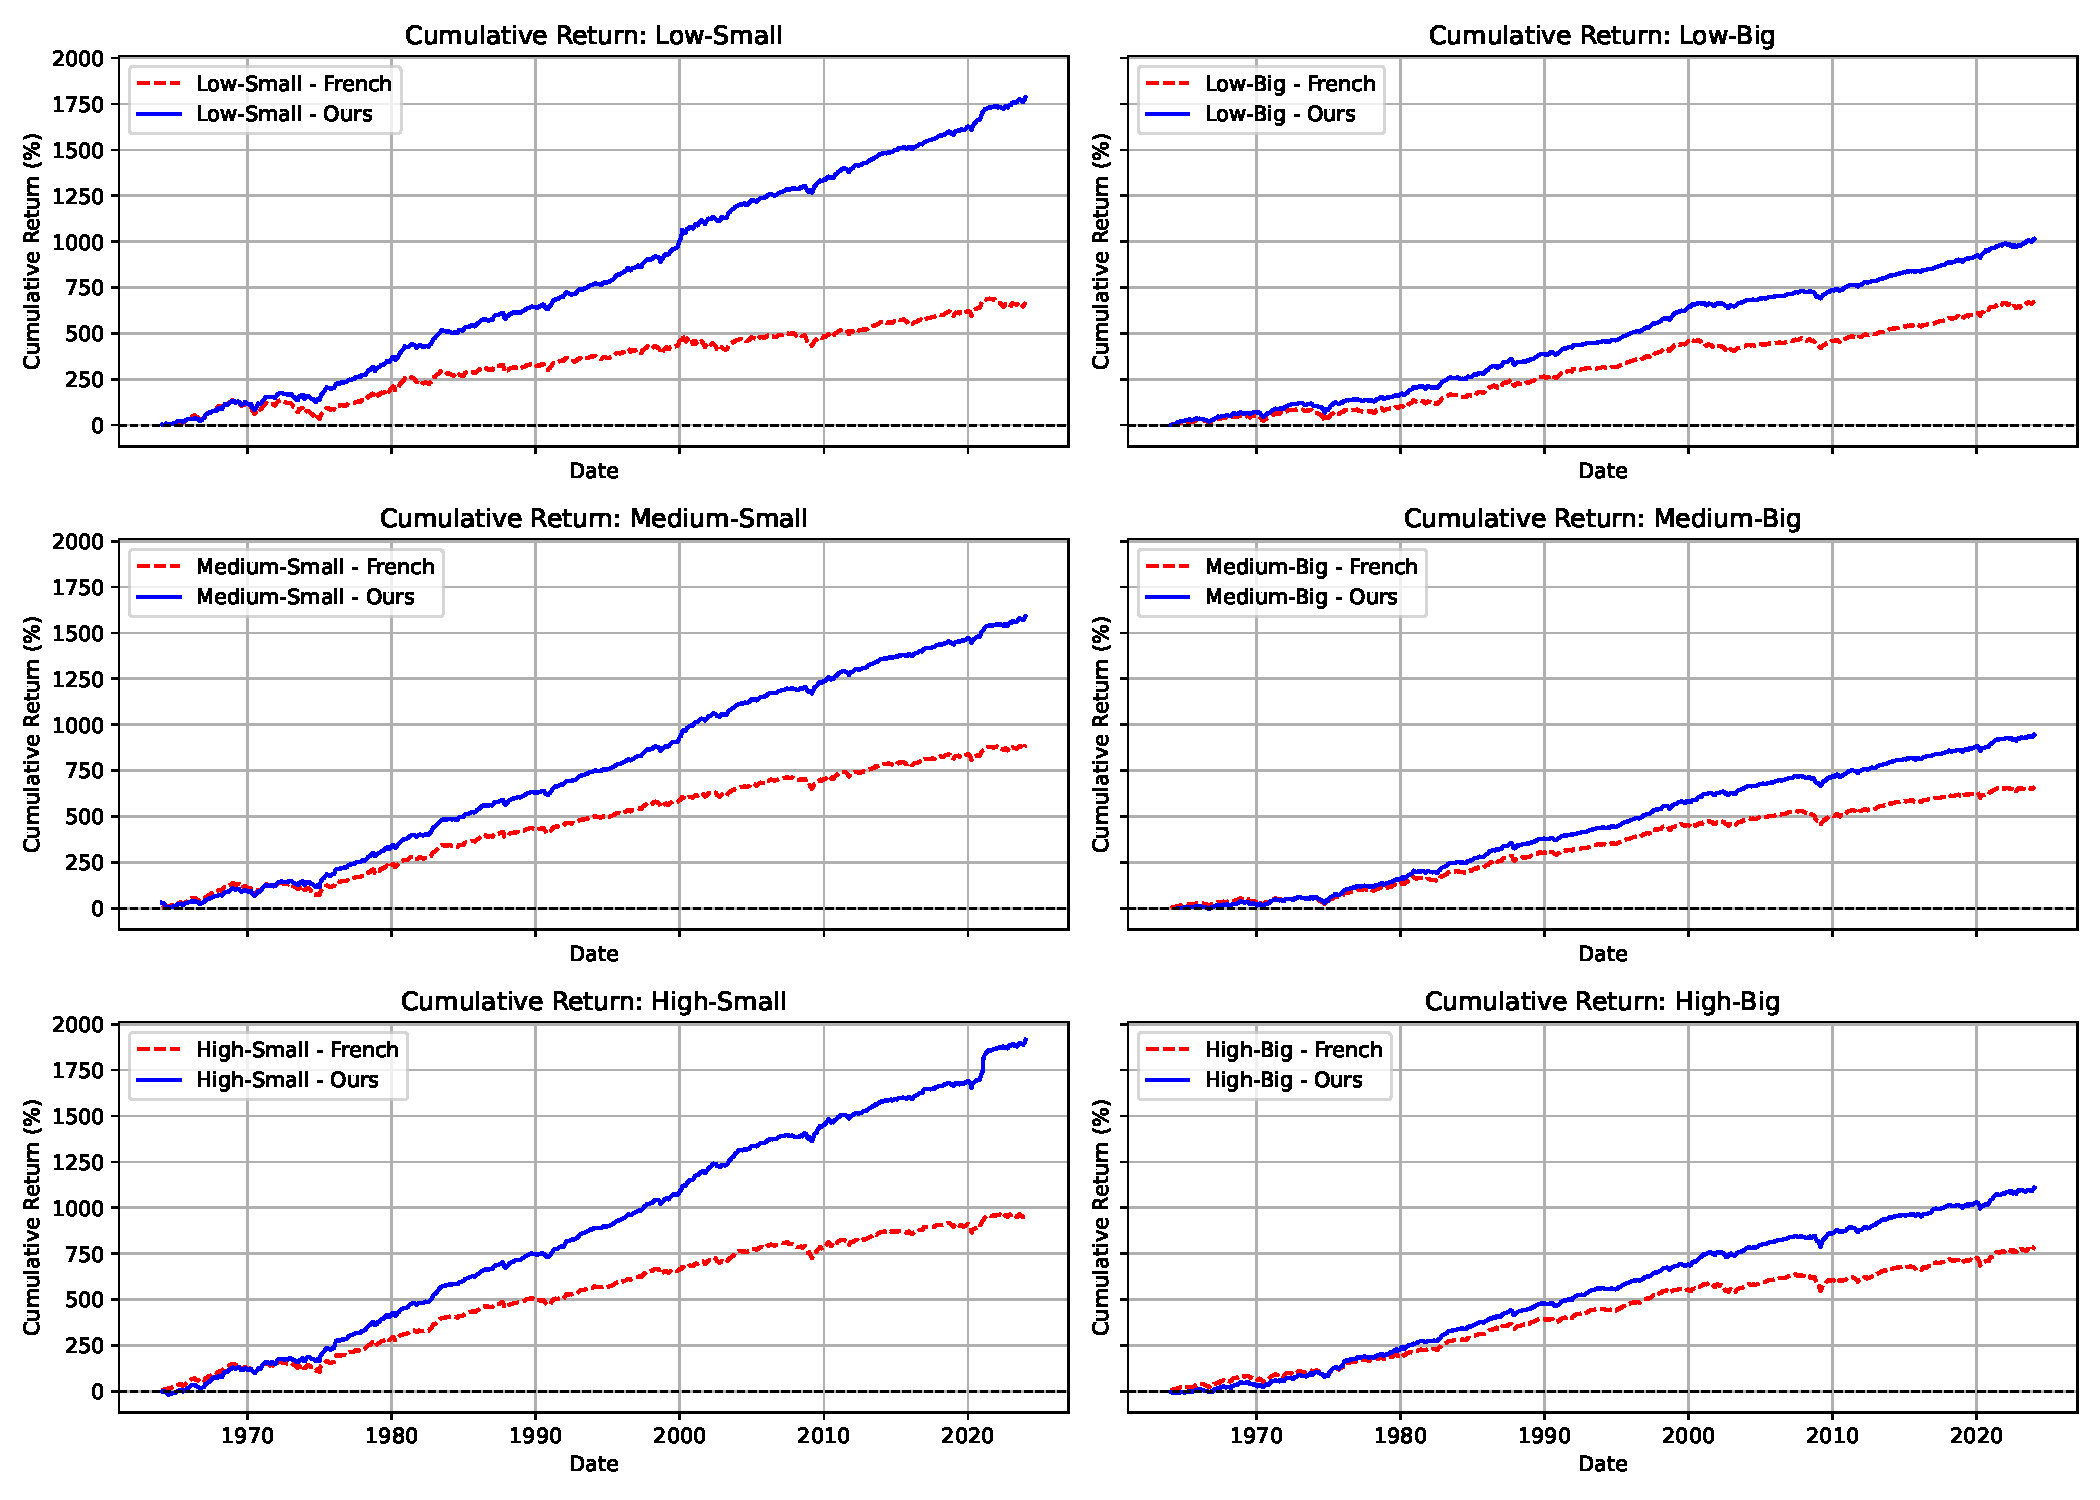
\includegraphics[width=1\linewidth]{../Plots/cumulative_returns.pdf}
\caption{Cumulative Returns of the French and Value-Weighted Portfolios.}
\label{fig:CRFVP}
\end{figure}

\section*{Exercise (\textit{ii})}

The vector of sample mean excess returns is illustrated in \autoref{tab:SME}.
It illustrates that the small firms have higher mean excess returns than the
big firms in our data. However, these excess returns for the small firms
come at a cost of higher volatility as displayed in \autoref{fig:CMVP}.

% The table of sample mean excess returns
\begin{table}[H]
\centering
\caption{Sample Mean Excess Returns of the Six Portfolios.}
\label{tab:SME}  
\begin{tabular}{ c c c c c c c c }
\toprule
Portfolio & Mean Excess Return (\%) \\
\midrule
Low Small & 2.12 \\
Medium Small & 1.85 \\
High Small & 2.30 \\
Low Big & 1.05 \\
Medium Big & 0.96 \\
High Big & 1.18 \\
\bottomrule
\end{tabular}    
\end{table}

\begin{figure}[H]
\centering
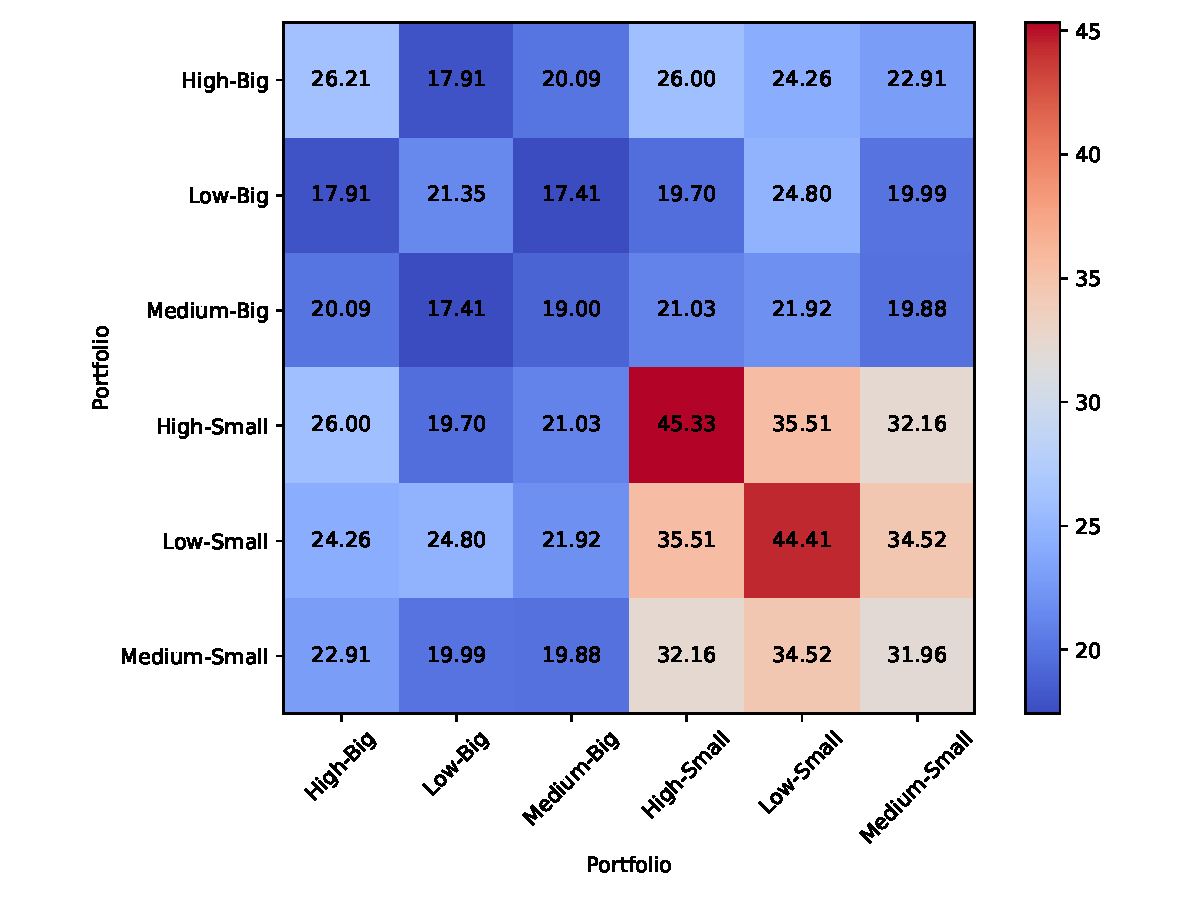
\includegraphics[width=1\linewidth]{../Plots/covariance_matrix.pdf}
\caption{Covariance Matrix of the Value-Weighted Portfolios.}
\label{fig:CMVP}
\end{figure}

In our data, the Sharpe ratio of the tangency portfolio and the market 
portfolio is approximately $0.36$ and $0.26$, respectively. Hence, our 
value-weighted market portfolio is not mean-variance efficient ex post. 
This suggests that, according to the mean variance framework, our proxy for 
the market portfolio does not achieve the optimal risk-adjusted return, 
potentially due to market frictions, data limitations, or deviations from 
CAPM. However, we observe from \autoref{fig:MVF} that the market portfolio is not 
mean-variance dominated by any of the four Fama-French portfolios. In that 
sense, there is still no free lunch; to obtain a higher return, one must 
also accept a higher risk. 

\begin{figure}[H]
    \centering
    \begin{subfigure}[b]{0.48\textwidth}
        \centering
        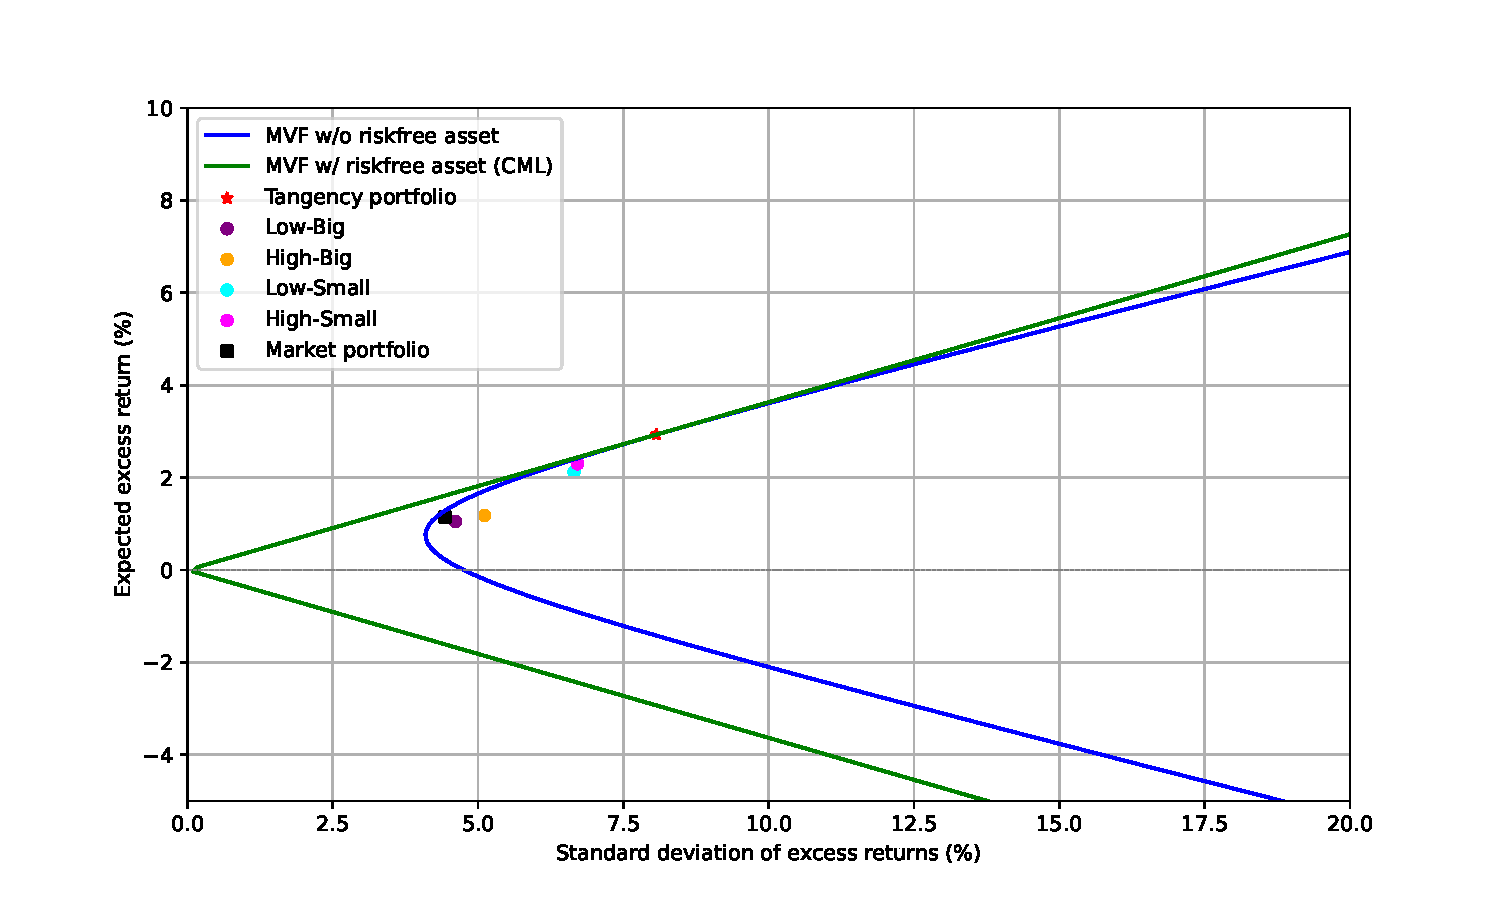
\includegraphics[width=\linewidth]{../Plots/ex_post_MVF.pdf}
        \caption{Mean Variance Frontiers with Four Portfolios.}
        \label{fig:MVF4}
    \end{subfigure}
    \hfill
    \begin{subfigure}[b]{0.48\textwidth}
        \centering
        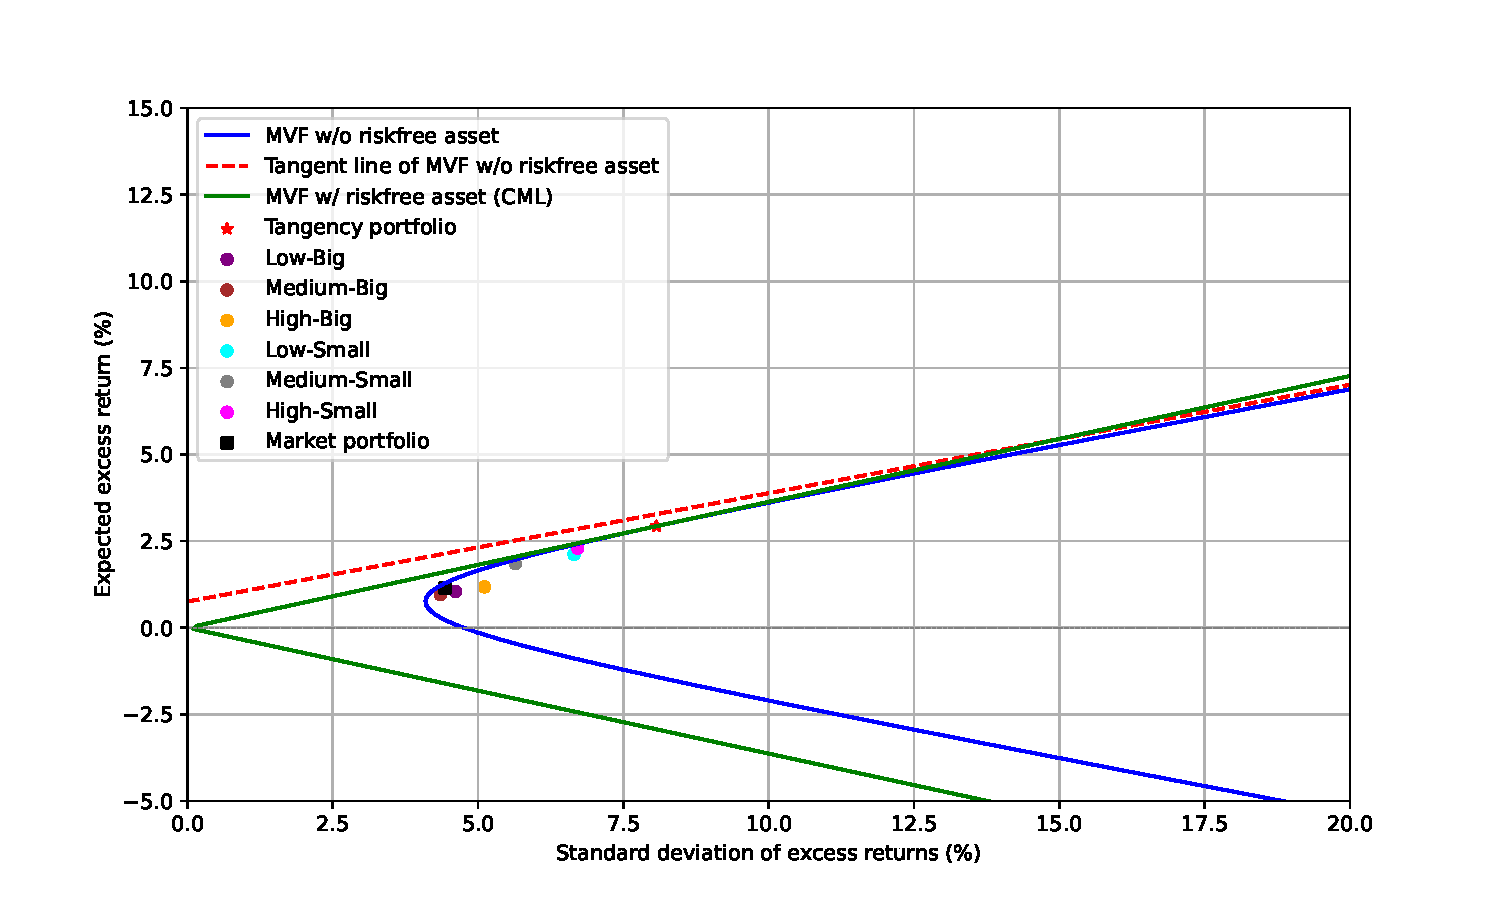
\includegraphics[width=\linewidth]{../Plots/ex_post_MVF_v2.pdf}
        \caption{Mean Variance Frontiers with Six Portfolios.}
        \label{fig:MVF6}
    \end{subfigure}
    \caption{Ex-Post Mean Variance Frontiers.}
    \label{fig:MVF}
\end{figure}

\section*{Exercise (\textit{iii}) \& (\textit{iv})}

From \autoref{fig:EPSML}, we find that the small firms have expected 
excess returns well above what would be justified from their betas alone, 
and hence exhibit positive alpha. On the other hand, the large firms have
have expected returns more in line with what would be expected 
from their betas, although the \textit{Low Big} portfolio have somewhat of 
a negative alpha. These visual results are further strengthened by the 
regressions presented in the \autoref{tab:RRSP}, which shows that the \textit{Low Small} and \textit{High Small} portfolios have 
positive alphas and the \textit{Low Big} portfolio a negative alpha. All in all, our 
results suggest that there is a size-related risk premium that is 
not accounted for by the CAPM. In particular, small firms are sold at a discount 
(undervalued) versus what would be predicted by the CAPM. In addition, there is some
evidence that large growth firms\footnote{\textit{Low Big} firms.} are sold at a
premium (overvalued) versus the large value firms\footnote{\textit{High Big} firms.}. 

\begin{figure}[H]
\centering
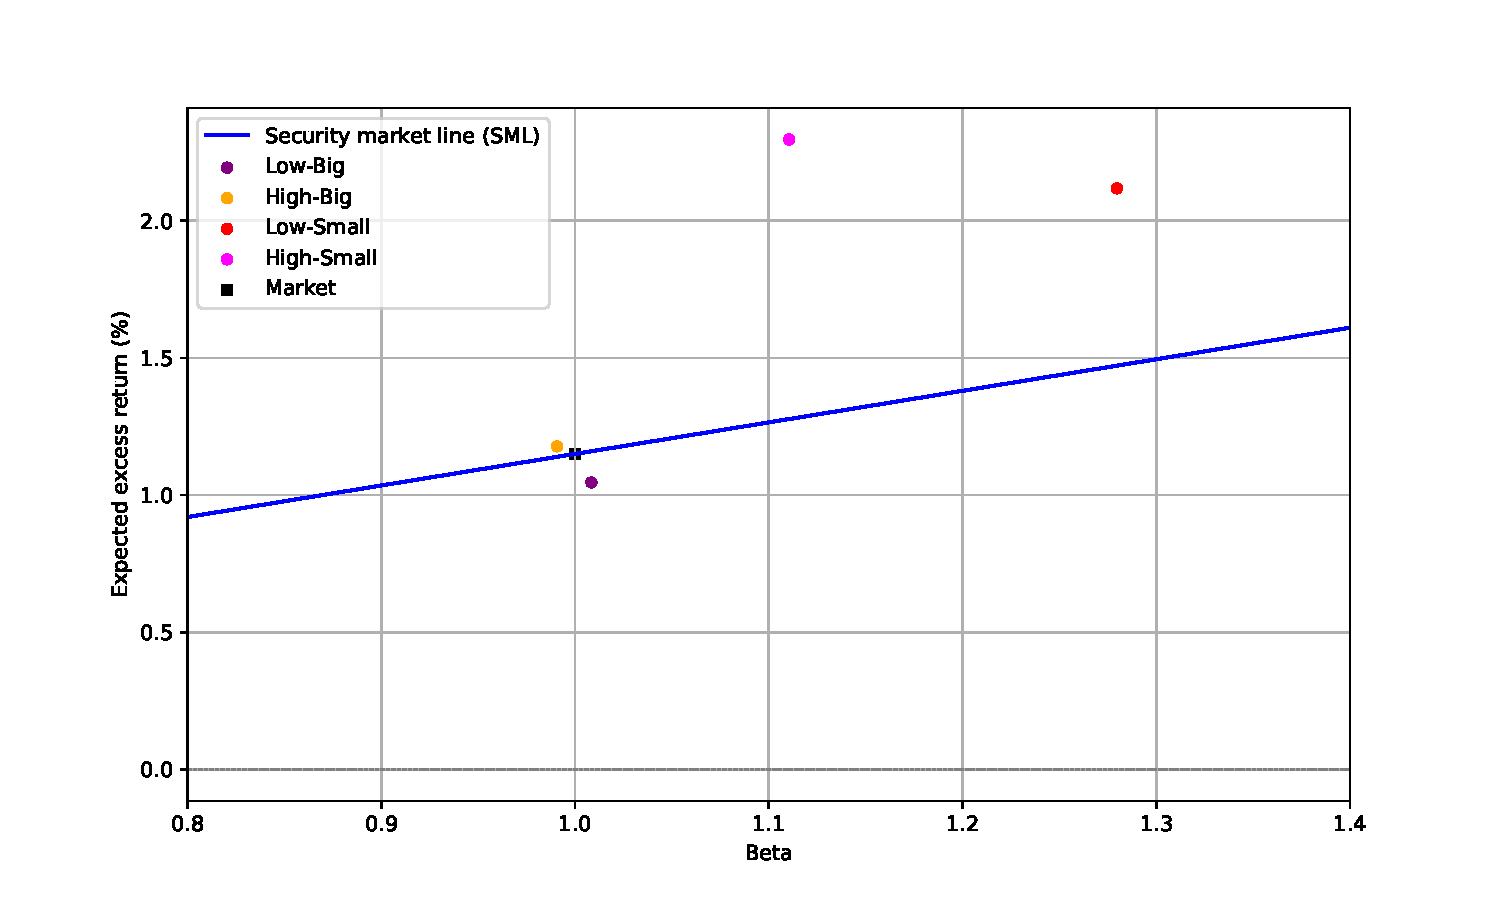
\includegraphics[width=0.95\linewidth]{../Plots/ex_post_SML.pdf}
\caption{Security Market Line.}
\label{fig:EPSML}
\end{figure}


\begin{table}[H]
    \centering
    \caption{Regression Results for the Four Portfolios.}
    \label{tab:RRSP}
    {
\def\sym#1{\ifmmode^{#1}\else\(^{#1}\)\fi}
\begin{tabular}{@{\extracolsep{2pt}}l*{4}{c}@{}}
\hline\hline


 & Low-Big & High-Big & Low-Small & High-Small \\
\hline
$\beta$ & 1.01\sym{**} & 0.99\sym{**} & 1.28\sym{**} & 1.11\sym{**} \\
 & (0.01) & (0.02) & (0.03) & (0.04) \\
$\alpha$ & -0.11\sym{**} & 0.04 & 0.65\sym{**} & 1.02\sym{**} \\
 & (0.04) & (0.10) & (0.13) & (0.18) \\

\hline
Obs & 720 & 720 & 720 & 720 \\
R\sym{2} & 0.94 & 0.74 & 0.73 & 0.54 \\
\hline\hline
\multicolumn{5}{l}{\footnotesize Standard errors in parantheses}\vspace{-.25em} \\
\multicolumn{5}{l}{\footnotesize *** p<0.001, ** p<0.005, * p<0.01}
\end{tabular}
}
\end{table}













\newpage
\bibliography{ref}


\end{document}